\documentclass[a11paper, 11pt]{article}

\usepackage{document}
\usepackage{titlepage}
\usepackage{float}
\usepackage{algorithm}
\usepackage{amsmath}
\usepackage{graphicx}
\usepackage{tikz-uml}
\usepackage{algpseudocode}
\usepackage{frpseudocode}
\usepackage[T1]{fontenc}
\usepackage[french]{babel}

% \addbibresource{bibliography.bib}
% \nofiles


% \institution{Université de Sherbrooke}
% \faculty{Faculté de génie}
% \department{Département de génie électrique et de génie informatique}
\title{Rapport d'APP}
\classnb{GEN241}
\class{Modélisation et programmation orientée objet}
\author{
  \addtolength{\tabcolsep}{-0.4em}
  \begin{tabular}{rcl} % Ajouter des auteurs au besoin
  Benjamin Chausse & -- & chab1704 \\
  \end{tabular}
}
\teacher{Domingo Palao Muñoz}
% \location{Sherbrooke}
% \date{\today}


\begin{document}
\maketitle
\newpage
\tableofcontents
\listoffigures
\listoftables
\newpage

\section{Diagrammes UML}

La figure \ref{fig:class} montre les diverses relation entre les classes de
graphicus-02. Elle permet d'observer la hiérarchie des classes ainsi que les
facteurs de dépendance entre les classes.

\begin{figure}[H] % Diagramme de classes {{{
\centering
\caption{Diagrame de classes de graphicus-02}\label{fig:class}
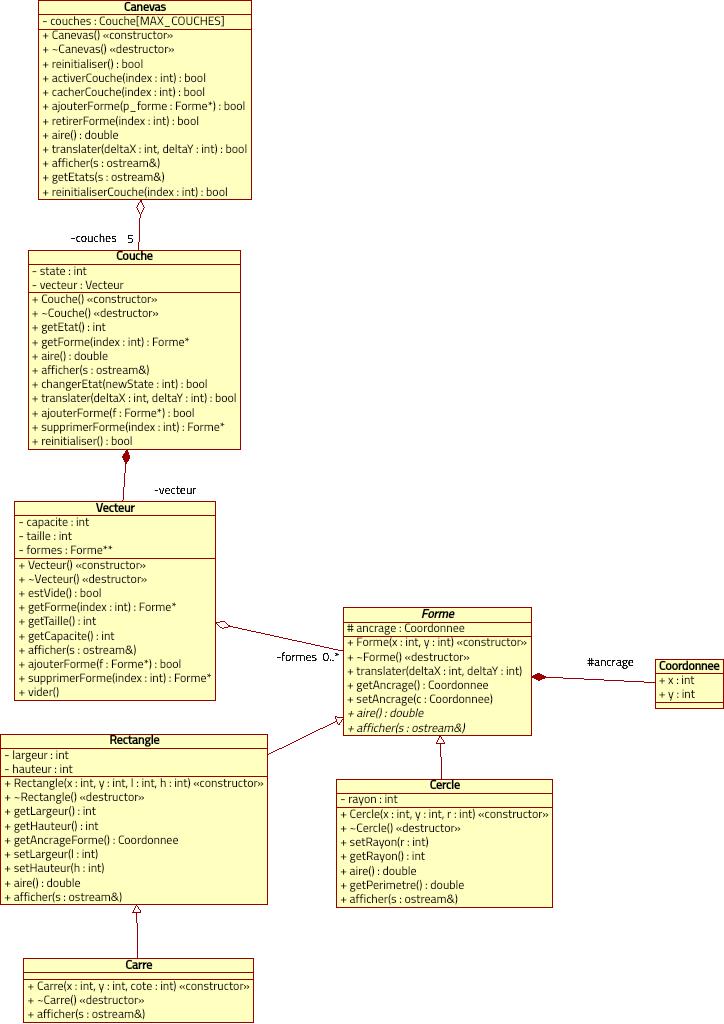
\includegraphics[width=0.8\textwidth]{class.png}
\end{figure} % }}}

La figure \ref{fig:sequence} montre comment l'application procéderait
lorsqu'un utilisateur voudrait activer la couche 1 du canevas alors que la
couche 0 est présentement active. Les autres couches ont été omises pour
alléger le diagramme.

\begin{figure}[H] % Diagramme de séquence {{{
\centering
\caption{Diagrame de séquence d'activation de couche}\label{fig:sequence}
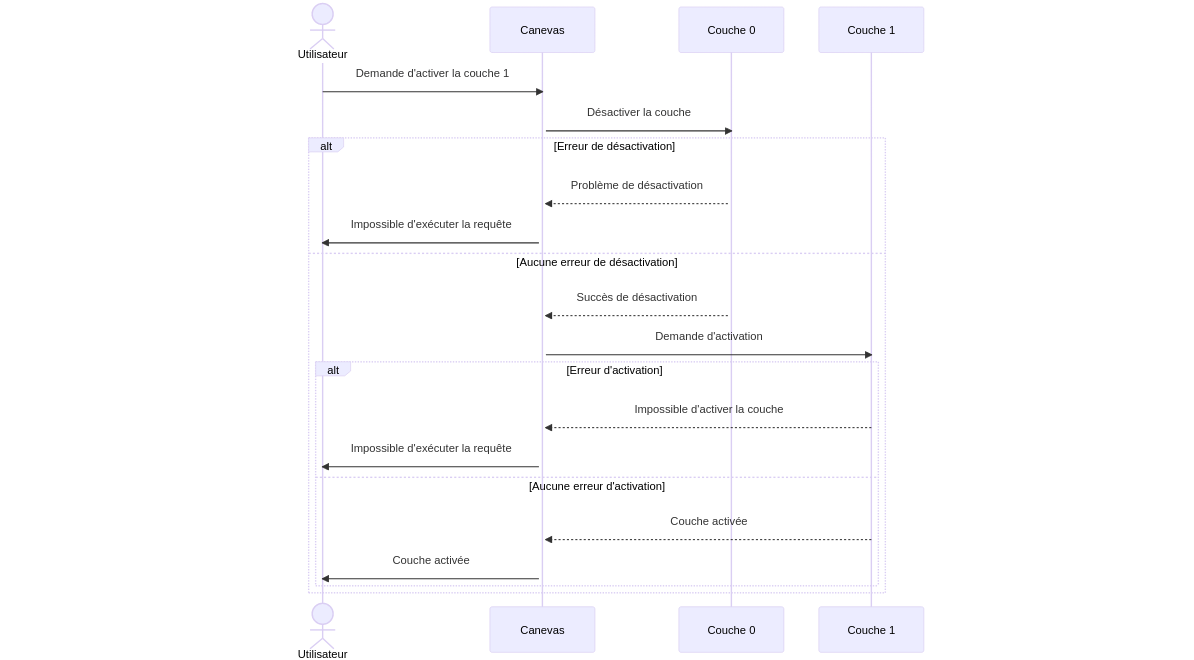
\includegraphics[width=\textwidth]{sequence.png}
\end{figure} % }}}


La figure \ref{fig:usecase} montre les différentes actions que l'utilisateur
peut exécuter dans l'application. Nous voyos par la suite comment certaines de
ces actions agissent en arrière plan et dépendent d'autres actions (parfois
même d'autres actions accessibles à l'utilisateur).

\begin{figure}[H]
\centering\caption{Diagramme de cas d'utilisation}\label{fig:usecase}
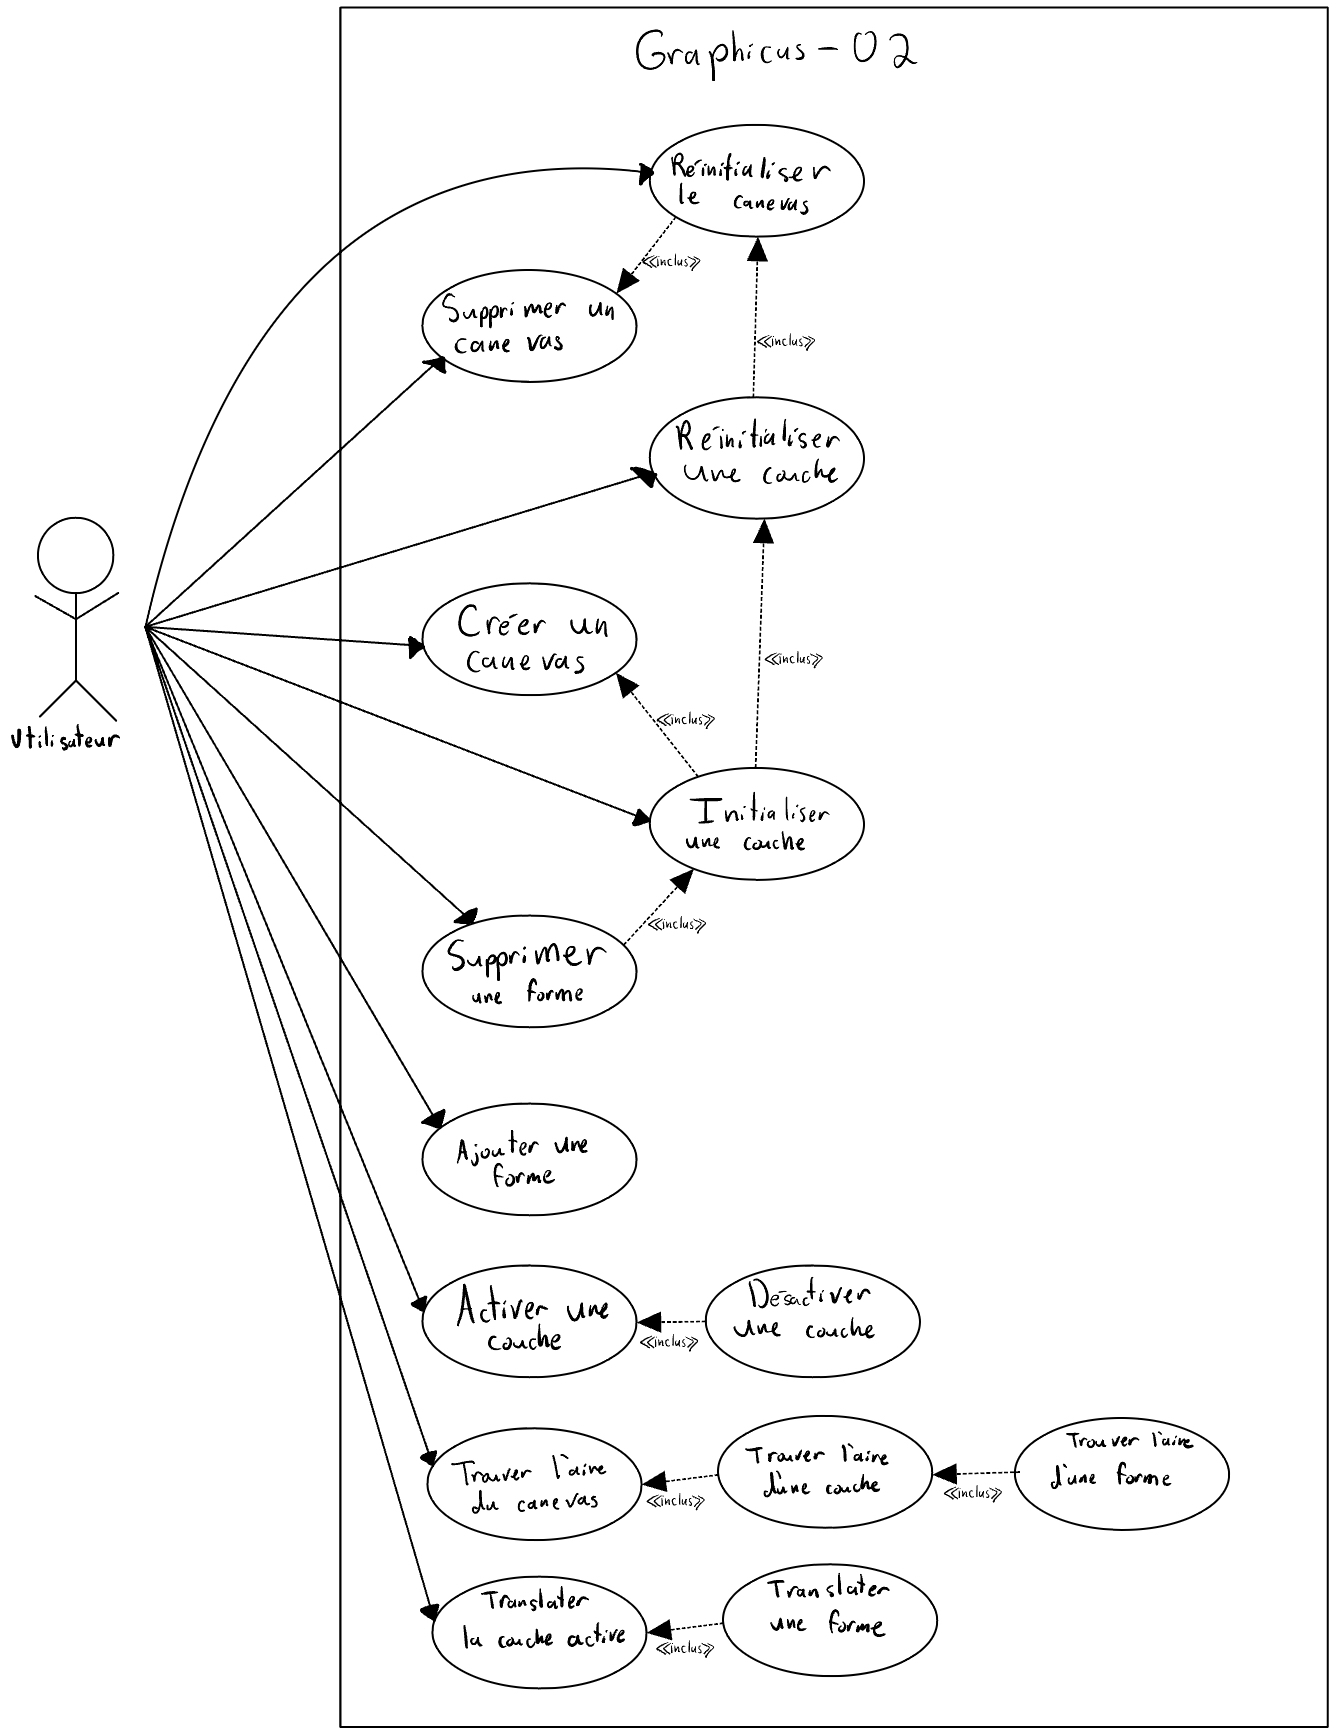
\includegraphics[width=\textwidth]{usecase.png}
\end{figure}


\section{Pseudo-code}

\begin{algorithm} % {{{
\caption{Ajout d'un élément au vecteur}\label{alg:ajouterForme}
\begin{algorithmic}[1]
  \Function{Vecteur::ajouterForme}{$f$}{ Booléen}\\
  \hspace{.5cm}// $f$: Forme à ajouter au vecteur\\
  \hspace{.5cm}// $Vecteur::taille$: nombre d'éléments actuellement dans le vecteur (entier)\\
  \hspace{.5cm}// $Vecteur::capacite$: capacité maximale du vecteur actuellement (entier)\\
  \hspace{.5cm}// $Vecteur::formes$: Liste de pointeurs vers les formes du vecteur (*Forme)\\
  \textbf{DÉBUT}\\
  \hspace{.5cm}// $newCapacite$: nouvelle capacité du vecteur (entier)\\
  \hspace{.5cm}// $newFormes$: nouvelle liste de pointeurs vers les formes du vecteur (*Forme)
  \If{$f$ est de valeur nulle}
    \Comment{Vérifier si la forme est valide}
    \State\Return{Faux}
  \EndIf
  \If{$Vecteur::taille =\joinrel= Vecteur::capacite$}
    \Comment{Si le vecteur est plein}
    \State $newCapacite := Vecteur::capacite\times2$
    \If{L'espace disponible en mémoire $<$ $newCapacite\times taille(Forme)$}
      \State\Return{Faux}
    \EndIf
    \State $newFormes :=\ $allouer$(newCapacite\times taille(Forme))$
    \For{\textbf{CHAQUE} Forme $i$ dans $Vecteur::formes$}
      \State $newFormes[i] := Vecteur::formes[i]$
    \EndFor
    \State $Vecteur::capacite := newCapacite$
    \State libérer$(Vecteur::formes)$
    \State $Vecteur::formes := newFormes$
  \EndIf
  \State $Vecteur::taille := Vecteur::taille + 1$
  \State $Vecteur::formes[Vecteur::taille] := f$
  \State \Return{Vrai}
  \EndFunction
\end{algorithmic}
\end{algorithm} % }}}

\section{Plan de test}

\subsection{Identification}
\begin{table}[H] % {{{
\centering\caption{Informations générales du plan de test}\label{fig:planTest}
\begin{tabular}{rl}
  \\ \toprule
  Nom:               & Scénario de test du rapport d'APP \\
  But:               & Vérifier les fonctionnalitées globales de graphicus-02\\
  Acteur principal:  & classe \verb|Test| \\
  Date de création:  & 2023-01-14 \\
  Auteur:            & Benjamin Chausse -- chab1704 \\
  Version:           & 1.0 \\
  \bottomrule
\end{tabular}
\end{table}% }}}

\subsection{Scénario}

\subsubsection{Préconditions}

\begin{itemize}
  \item Un canevas vierge vient d'être créé
  \item Ce cas d'utilisation emploie la méthode \verb|tests_application_cas_02|
    de la classe \verb|Tests|. La première ayant été utilisée lors de la
    validation en classe.
\end{itemize}


\subsubsection{Postconditions}

\begin{itemize}
  \item Le déroulement du test se fait sans intervention de l'utilisateur.
  \item L'affichage doit-être accessible à l'évaluateur:
      \begin{itemize}
        \item soit par écriture dans un fichier
        \item soit par affichage dans un terminal
      \end{itemize}
  \item Le numéro de chaque étape est identifié avant son exécution.
  \item La description de chaque étape est affichée avant son exécution.
  \item Les informations passées à chaque étape sont affichées avant son exécution.
\end{itemize}


\subsubsection{Limitations}

\begin{itemize}
  \item Le test ne vérifie pas la totalité des cas limites
    (ex: capacité insuffisante en mémoire pour agrandir le vecteur).
\end{itemize}


\subsection{Enchaînement nominal}

\subsubsection{Étapes 1 à 4}
\begin{enumerate}
  % \setcounter{enumi}{1}
  \item Activer la couche d'index 4
  \item Ajouter les formes suivantes au canevas:
    \begin{itemize}
      \item un cercle de centre (1, 2) et de rayon $\frac{1}{\sqrt{\pi}}$
      \item un rectangle anchré en (3, 4), de dimensions $3\times4$
      \item un carré anchré en (-1, -1), de côté 2
    \end{itemize}
  \item Afficher le canevas
  \item Imprimer l'aire du canevas (doit être égale à $1+12+4$ soit $17$)
\end{enumerate}

\subsubsection{Étapes 5 à 13}
\begin{enumerate}
  \setcounter{enumi}{4}
  \item Activer la couche d'index 3
  \item Ajouter les formes par défaut au canevas. Soit:
  \begin{itemize}
    \item un cercle de centre (0, 0) et de rayon 1
    \item un rectangle anchré en (0, 0), de largeur 1 et de hauteur 1
    \item un carré anchré en (0, 0), de côté 1
  \end{itemize}
  \item Afficher le canevas
  \item Translater la couche active de (1, 1)
  \item Afficher le canevas
  \item Supprimer la forme de l'index 0 (la première)
  \item Activer la couche d'index 4
  \item Supprimer la forme de l'index 2 (la dernière)
  \item Afficher le canevas
\end{enumerate}
\subsubsection{Étapes 14 à 18}
\begin{enumerate}
  \setcounter{enumi}{13}
  \item Initialiser la couche d'index 4
  \item Afficher le canevas
  \item Imprimer l'aire du canevas (doit être égale à $1+1$ soit $2$)
  \item Réinitialiser le canevas
  \item Afficher le canevas
\end{enumerate}


% \newpage
% \printbibliography[heading=bibintoc]
\end{document}
